\documentclass[thesis]{subfiles}

\begin{document}

\chapter{Foundations}
\label{chapter:foundations}

Before introducing \pyop3, it is instructive to review its `foundations', that is, pieces of software that have inspired its design.
In order these are: \numpy, PETSc DMPlex and \pyop2.

\section{A language for structured data: \numpy}

As we have established in \cref{chapter:introduction}, data structures for mesh-based computations have a non-trivial hierarchical structure that existing mesh stencil packages are incapable of representing in full.
Prior to introducing \pyop3's abstraction for handling this (\emph{axis trees}, \cref{chapter:axis_trees}) it is valuable to examine existing techniques for handling hierarchically structured data.
To that end we will review \numpy, the de-facto package for array-based computation in Python~\cite{harrisArrayProgrammingNumPy2020}.
In addition to considering implementation details, elements of \numpy's interface will be presented since, given \numpy's ubiquity and the fact that \pyop3 is a Python DSL, \pyop3 aims to reuse as much of its terminology and syntax as possible.

\subsection{N-dimensional arrays}

\begin{figure}
  \centering

  \begin{subfigure}{.4\textwidth}
    \centering
    \includegraphics{numpy_ndarray.pdf}
  \end{subfigure}
  %
  \begin{subfigure}{.58\textwidth}
    \centering
    \begin{tblr}{|[1pt]l|[1pt]l|[1pt]}
      \hline[1pt]
      \texttt{data} & \texttt{0x7ff...} \\
      \hline
      \texttt{data type} & \texttt{int32} \\
      \hline
      \texttt{shape} & \texttt{(2, 3, 2)} \\
      \hline
      \texttt{strides} & \texttt{(24, 8, 4)} \\
      \hline[1pt]
    \end{tblr}
    \vspace{2em}
  \end{subfigure}

  \caption{
    The data layout (left) and internal representation (right) of an \pycode{int32} \numpy array with shape \pycode{(2, 3, 2)}.
    Strides are given in bytes for each axis.
  }
  \label{fig:numpy_ndarray}
\end{figure}

In \numpy, hierarchical data is represented by \emph{N-dimensional arrays}.
These have a multi-level \emph{shape}, with each level called an \emph{axis} (e.g. \cref{fig:numpy_ndarray}, left).

In order to access a value from the array a \emph{multi-index} - a list of integers, one per axis - must be provided.
Given a multi-index, the correct value may be read from the array by computing an offset and then accessing the data at that offset.
The function used to compute this offset is a function of each multi-index, for example, for the array shown in \cref{fig:numpy_ndarray}, the offset is given by

\begin{equation*}
  \textnormal{offset}(i_0, i_1, i_2) = 6 i_0 + 2 i_1 + i_2
\end{equation*}

\noindent
where $i_0$, $i_1$, and $i_2$ are the values of the multi-index for axes 0, 1, and 2 respectively.
The Python syntax for performing this access would be \pycode{array[i0, i1, i2]}.

To represent arrays, \numpy internally combines a memory buffer, containing the actual values, with additional \emph{metadata} used to interpret the buffer.
In particular, the metadata includes the \emph{shape} of the array, how to \emph{stride} through it, and its data type (e.g. \cref{fig:numpy_ndarray}, right).
Representing data in this way allows array transformations to be expressed without needing to copy data.
Arrays can be reshaped or transposed just by constructing a new metadata struct with alternative shape and/or stride information.
These alternative representations for the same array are termed \emph{views}.

\subsection{Indexing arrays}
\label{sec:numpy_indexing_arrays}

\begin{table}
  \begin{tblr}{|[1pt]l|[1pt]l|[1pt]l|[1pt]l|[1pt]}
    \hline[1pt]
    \textbf{Index operation} & \textbf{Example} & \textbf{Return value} & \textbf{Array return type} \\
    \hline[1pt]
    Slicing & \pycode{array[1:6:2]} & \pycode{["B", "D", "F"]} & View \\
    \hline
    Integer array indexing & \pycode{array[[0, 3, 4]]} & \pycode{["A", "D", "E"]} & Copy \\
    \hline[1pt]
  \end{tblr}
  \caption{
    Important indexing operations for \numpy arrays.
    The examples shown apply the index to the string array \pycode{["A", "B", "C", "D", "E", "F"]} (called \pycode{array} above).
  }
  \label{tab:numpy_indexing_ops}
\end{table}

In addition to reshaping, arrays may also be \textit{indexed}, where portions of the full array are extracted to yield a new array.
For \pyop3 the most relevant indexing operations (demonstrated in \cref{tab:numpy_indexing_ops}) are:

\begin{description}
  \item[Slicing]
    For affine indexing operations one can pass a Python \pycode{slice} object to index an axis.
    One can index an axis of an array with the syntax \pycode{[start:stop:step]}, where omitting \pycode{start}, \pycode{stop} or \pycode{step} will default to 0, the end of the array, and 1 respectively.
    Due to the regular access pattern of a slice, indexing \numpy arrays with them will return a view.

  \item[Integer array indexing]
    For irregular access patterns, an array of indices may be used to select entries from a given axis.
    In contrast with slices, this method is inherently irregular and so a copy of the array is returned, instead of a view.
\end{description}

\section{Relating unknowns to mesh topology: PETSc DMPlex}
\label{sec:foundations_dmplex}

As previously mentioned, existing abstractions for mesh data typically fall short in one of two ways.
They either:
(a) assume that DoFs belong to a single entity type, or
(b) delegate responsibility for handling the mesh entirely to the user and instead deal with the more abstract concept of \emph{nodes}.

\begin{figure}
  \centering
  \begin{subfigure}{.49\textwidth}
    \centering
    \includegraphics{two_cell_mesh.pdf}
  \end{subfigure}
  %
  \begin{subfigure}{.49\textwidth}
    \centering
    \includegraphics{dmplex_hasse.pdf}
  \end{subfigure}
  \caption{
    The Hasse diagram (right) for a two-cell mesh (left).
  }
  \label{fig:dmplex_hasse}
\end{figure}


One piece of software offering a solution to this dilemma is DMPlex~\cite{knepleyMeshAlgorithmsPDE2009,knepleyUnstructuredOverlappingMesh2015,langeEfficientMeshManagement2016}, the unstructured mesh component of PETSc~\cite{petsc-efficient,petsc-user-ref,petsc-web-page}.
DMPlex represents meshes as directed acyclic graphs (DAGs) where mesh entities, termed \emph{points}, are the vertices of the graph and entity covering relations are its edges (e.g. cells connect to facets).
Since the DAG forms a partially-ordered set, it is common to visualise DMPlex instances as Hasse diagrams (\cref{fig:dmplex_hasse}).
All entities with the same topological dimension are shown as different layers, or \emph{strata}, of the diagram.

By treating mesh entities equivalently, DMPlex is able to express mesh algorithms generically (e.g. parallel mesh distribution~\cite{knepleyUnstructuredOverlappingMesh2015}, checkpointing~\cite{hamEfficientNtoMCheckpointing2024}) in an entirely dimension-independent fashion.
Also, importantly, representing (interleaved) mesh data storing DoFs on different entities becomes trivial (\cref{sec:dmplex_data_layout}).

It is this `dual' representation of mesh entities - as `flat' points and as a set of relations - that makes DMPlex so effective, and hence is an abstraction that we wish to represent in \pyop3.
Indeed, in places the similarities between DMPlex's and \pyop3's abstractions are so strong that \textbf{one can consider \pyop3 to be the abstraction that automates DMPlex.}

\subsection{Topological queries}

\begin{figure}
  \centering
  \begin{subfigure}{.49\textwidth}
    \centering
    \includegraphics{dmplex_hasse_cone.pdf}
    \caption{cone: $\cone(0) = \{6,7,8\}$}
  \end{subfigure}
  %
  \begin{subfigure}{.49\textwidth}
    \centering
    \includegraphics{dmplex_hasse_support.pdf}
    \caption{support: $\support(8) = \{0,1\}$}
  \end{subfigure}

  \vspace{1em}

  \begin{subfigure}{.49\textwidth}
    \centering
    \includegraphics{dmplex_hasse_closure.pdf}
    \caption{closure: $\plexclosure(0) = \{0,6,7,8,2,3,4\}$}
  \end{subfigure}
  %
  \begin{subfigure}{.49\textwidth}
    \centering
    \includegraphics{dmplex_hasse_star.pdf}
    \caption{star: $\plexstar(3) = \{3,7,8,9,0,1\}$}
  \end{subfigure}

  \caption{
    The possible DMPlex covering queries applied to the mesh from \cref{fig:dmplex_hasse}.
  }
  \label{fig:dmplex_queries}
\end{figure}

To traverse the DAG and build appropriate stencils, DMPlex provides two core topological query operations: \emph{cone} and \emph{support}.
The cone of a point, written $\cone(p)$, is the set of points that are pointed to from $p$.
The support of a point, written $\support(p)$, is the dual of cone and yields the set of points that point to $p$.
Transitive closures for both of these operations, where the operation is applied repeatedly and all points are accumulated, are also supplied by DMPlex.
The transitive closure of cone is termed the \emph{closure} ($\plexclosure(p)$) and the transitive closure of support is called the \emph{star} ($\plexstar(p)$).
These operations are shown in \cref{fig:dmplex_queries}.

It is possible to compose these operations to yield larger stencils.
For instance $\support(\cone(p))$ with $p$ a cell produces the set of cells sharing an edge with $p$ (and $p$ itself).
Likewise, $\plexclosure(\plexstar(p))$ is the \textit{adjacency} relation for finite element calculations: basis functions on points within this stencil have non-zero support with the basis functions on $p$.

\subsection{Representing data layouts}
\label{sec:dmplex_data_layout}

\begin{listing}
  \centering

  \caption{
    C code constructing an appropriate \ccode{PetscSection} for a $[P_3]^2$ finite element (\cref{fig:scott_vogelius_element_P3}).
    Some boilerplate code is omitted.
  }

  \begin{minipage}{.9\textwidth}
    \begin{calgorithm}
      // set cell DoFs (2 per cell)
      DMPlexGetDepthStratum(dmplex, 2, &start, &end);
      for (int cell=start; cell<end; cell++)
        PetscSectionSetDof(section, cell, 2);

      // set edge DoFs (4 per edge)
      DMPlexGetDepthStratum(dmplex, 1, &start, &end);
      for (int edge=start; edge<end; edge++)
        PetscSectionSetDof(section, edge, 4);

      // set vertex DoFs (2 per vertex)
      DMPlexGetDepthStratum(dmplex, 0, &start, &end);
      for (int vertex=start; vertex<end; vertex++)
        PetscSectionSetDof(section, vertex, 2);

      PetscSectionSetUp(section);
    \end{calgorithm}
  \end{minipage}

  \label{listing:section_p3}
\end{listing}

\begin{algorithm}
  \caption{
    The tabulation algorithm that determines the right offsets from a \ccode{PetscSection}.
    This code is executed during \ccode{PetscSectionSetUp()}.
  }

  \begin{algorithmic}[1]
    \Require \textit{permutation}
    \State \textit{counter} $\gets$ 0
    \State \textit{offset} $\gets$ 0
    \For{\textit{point} \textbf{in} \textit{mesh.points}}
      \State \textit{offsets}[\textit{counter}] = \textit{offset}
      \State \textit{counter} $\gets$ \textit{counter} + 1
      \State \textit{renumbered} $\gets$ \textit{permutation}[\textit{point}]
      \State \textit{offset} $\gets$ \textit{offset} + \Call{PetscSectionGetDof}{\textit{renumbered}}
    \EndFor
  \end{algorithmic}

  \label{alg:petsc_section_tabulate}
\end{algorithm}

In order to associate data with DMPlex points users must construct a \ccode{PetscSection}, a simple CSR-like data structure that associates mesh points with offsets into an array.
To build one, a number of DoFs must be associated with each mesh point before calling \ccode{PetscSectionSetUp()} (shown in \cref{listing:section_p3}).
This last step traverses the input points and accumulates the offset for each point, building the array that may then be queried later on (\cref{alg:petsc_section_tabulate}).
To give a simple example, given the \gls{dof} count \ccode{[1, 0, 3, 2, 0, 1]} the \ccode{PetscSection} would tabulate the offsets to be \ccode{[0, 1, 1, 4, 6, 6]}.

\ccode{PetscSections} are able to express the renumbering locality optimisations described in \cref{sec:intro_mesh_numbering}.
One simply provides the \ccode{PetscSection} with an optional \emph{permutation} that is accounted for during set up.
This is demonstrated in \cref{alg:petsc_section_tabulate}.

\subsubsection{Limitations}

Whilst a powerful and flexible tool for describing data layouts, \ccode{PetscSections} have a number of shortcomings:

\begin{description}
  \item[They are fully ragged]
    \ccode{PetscSections} do not distinguish between different types of topological entity and so important structure cannot be represented.
    They only store DoF information per point in a completely unstructured way and are incapable of knowing, say, that every cell in the mesh stores exactly one DoF.
    This can prohibit the compiler from making certain optimisations (e.g. loop unrolling) with important performance implications.
    Further, not knowing the loop sizes a priori means that an additional array needs to be passed about during the calculation, directly harming the performance of memory-bound codes.

  \item[Shape information is lost]
    Though \ccode{PetscSections} allow one to directly associate DoFs with mesh entities of different dimension, they still lose information about the structure of the function space.
    For instance, to a \ccode{PetscSection}, a point with a single vector-valued node is indistinguishable from a point with multiple nodes.
\end{description}

\subsection{Parallel}
\label{sec:dmplex_parallel}

\begin{figure}
  \centering
  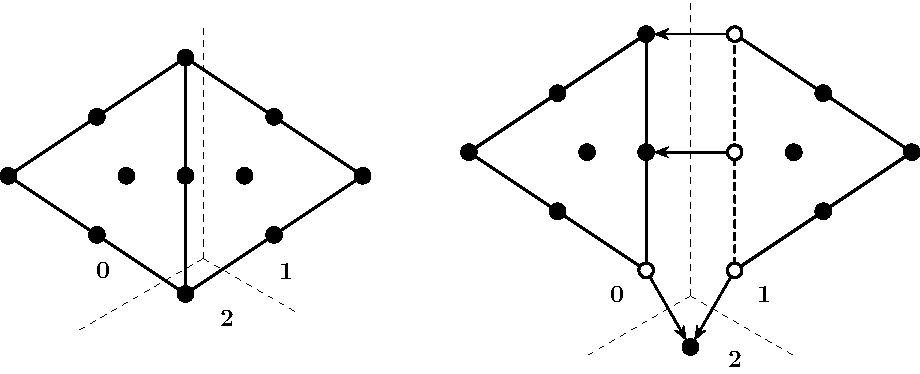
\includegraphics{star_forest_point.pdf}
  \caption{
    Global (left) and process-local (right) views of a mesh partitioned between three processes.
    The black dots represent the different mesh entities (the \emph{points}).
    Ghost points are shown as hollow circles.
  }
  \label{fig:dmplex_split_mesh}
\end{figure}

As touched upon in \cref{sec:intro_???}, DMPlex works in distributed memory environments by partitioning the entire `global' mesh into local pieces that are kept on each process.
To enable stencil calculations \emph{ghost} points are duplicated across processes.
An example partitioned mesh is shown in \cref{fig:dmplex_split_mesh}.

\begin{figure}
  \centering
  \begin{subfigure}[t]{.45\textwidth}
    \centering
    \includegraphics{star_forest_abstract_mesh.pdf}
    \caption{Star forest suitable for describing the point sharing in \cref{fig:dmplex_split_mesh}.}
    \label{fig:star_forest_abstract_mesh}
  \end{subfigure}
  \hspace{1em}
  \begin{subfigure}[t]{.45\textwidth}
    \centering
    \includegraphics{star_forest_abstract_global.pdf}
    \caption{Star forest appropriate for storing the communication pattern of a globally consistent value.}
    \label{fig:star_forest_abstract_global}
  \end{subfigure}
  \caption{
    Common star forest patterns.
    Each point is labelled with its owning process and root and leaf points are shown in black and white respectively.
  }
\end{figure}

Parallel communication in DMPlex is handled by \textit{star forests}~\cite{zhangPetscSFScalableCommunication2021}.
Star forests relate equivalent points across processes as a collection (forest) of depth-1 trees (stars) consisting of a single \emph{root} and any number of \emph{leaves}.
They support two main operations: \emph{broadcasts} from roots to leaves and \emph{reductions} from leaves to roots.

Star forests are a powerful abstraction for describing a range of different parallel communication patterns.
For example,  a value shared globally across $n$ ranks can be represented as a star forest containing a single star with the root node on rank 0 and $n-1$ leaves, 1 for each other rank (\cref{fig:star_forest_abstract_global}).
For distributed meshes, star forests encode point ownership by making each shared point into a separate star, with the owning rank the root and ghost ranks the leaves.
A sketch of the star forest needed for \cref{fig:dmplex_split_mesh} is shown in \cref{fig:star_forest_abstract_mesh}.
In DMPlex this object is referred to as the \emph{point star forest}.

\begin{figure}
  \centering
  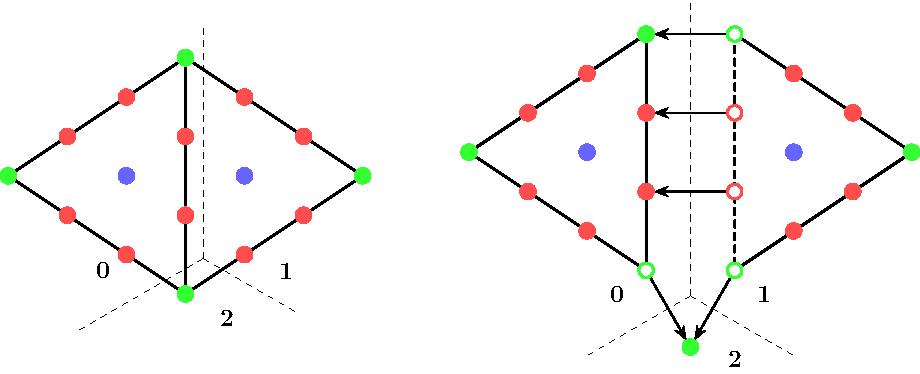
\includegraphics{star_forest_dof.pdf}

  \caption{
    Global (left) and process-local (right) views of a $P_3$ function space partitioned between three processes.
    Ghost DoFs are shown as hollow circles.
  }
  \label{fig:dmplex_split_function_space}
\end{figure}

In order to represent the parallel overlap of \emph{DoFs}, instead of points, a new star forest needs to be created.
To produce it, DMPlex composes the point star forest with the \ccode{PetscSection} encoding the function space.
This results in a \emph{DoF star forest} like that shown in \cref{fig:dmplex_split_function_space}.

\section{PyOP2}

% NOTE: should mention extruded (then mention at end of doc)

As first introduced in \cref{sec:intro_existing_software}, PyOP2 is a library for doing mesh stencil calculations~\cite{rathgeberPyOP2HighLevelFramework2012}.
It was originally introduced to provide the same abstractions as OP2~\cite{mudaligeOP2ActiveLibrary2012}, but using runtime code generation instead of source-to-source translation.
It is a core component of the Firedrake finite element framework~\cite{FiredrakeUserManual}.

\subsection{Data structures}

\begin{table}
  \centering
  \begin{tblr}{|[1pt]l|[1pt]l|[1pt]l|[1pt]l|[1pt]}
    \hline[1pt]
    & \textbf{Global} & \textbf{Dat} & \textbf{Mat} \\
    \hline[1pt]
    Usage & Globally constant value & Distributed vector & Distributed matrix \\
    \hline
    Constructor & \pycode{GlobalDataSet} & \pycode{DataSet} & 2 \pycode{DataSets} \\
    \hline
    Storage type & \numpy \pycode{ndarray} & \numpy \pycode{ndarray} & PETSc \ccode{Mat} \\
    \hline[1pt]
  \end{tblr}
  \caption{\pyop2 data structures.}
  \label{tab:pyop2_data_types}
\end{table}

Like \numpy, \pyop2 data structures are composed of a semi-opaque piece of memory and a data layout descriptor providing semantic information about said memory.
This data layout descriptor, termed a \emph{data set}, is constructed by taking a set, say, of vertices and associating some shape information with it.

Summarised in \cref{tab:pyop2_data_types}, \pyop2 has three supported data structures: \pycode{Globals} (constants), \pycode{Dats} (vectors), and \pycode{Mats} (matrices).
Each is constructed with a different data layout specification: \pycode{Globals} take a \pycode{GlobalDataSet}, \pycode{Dats} take a \pycode{DataSet}, and \pycode{Mats} take two \pycode{DataSets}, one each for the rows and columns.

\pycode{Globals} and \pycode{Dats} both store data as \numpy arrays under the hood, whereas \pycode{Mats} use PETSc matrices (also termed \ccode{Mats}).

For multi-field problems such as the Stokes example in \cref{chapter:introduction} one has \textit{mixed data sets}, which are simply a collection of regular data sets.
Mixed data sets yield \pycode{MixedDats} which are, again, simply a collection of regular \pycode{Dats}.
An example of a \pyop2 data layout for a multi-field problem is shown in \cref{fig:scott_vogelius_element_dof_layout_pyop2}.
Observe that, since the DoFs are associated with multiple mesh entities, data is stored on a \emph{node set}, losing topological information (\cref{sec:pyop2_limitations}).

\subsection{Parallel loops}

\begin{listing}
  \centering
  \begin{minipage}{.9\textwidth}
    \begin{pyalg2}
      par_loop(kernel,                          # local kernel
               src_set,                         # iteration set
               dat0(READ, src_to_target_map),   # arguments
               dat1(WRITE, src_to_target_map))
    \end{pyalg2}
  \end{minipage}
  \caption{
    Code to construct and execute a \pyop2 parallel loop.
  }
  \label{listing:pyop2_parloop_demo}
\end{listing}

In order to apply kernels to these data structures, a \textit{parallel loop} is constructed and executed.
The loop takes as arguments a \textit{local kernel}, \textit{iteration set} and zero or more \textit{arguments} that provide the data structures needed by the local kernel.
For an example parloop see \cref{listing:pyop2_parloop_demo}.

\begin{itemize}
  \item
    \pycode{kernel} is the local kernel representing the stencil operation to be performed per iteration.
    It may be either a string of C code or a \textit{loopy kernel} (see \cref{sec:pyop2_codegen}).
  \item
    \pycode{src_set} is the set that is iterated over.
  \item
    \pycode{dat0} and \pycode{dat1} are \pycode{Dat} objects (vectors) that are passed through to the local kernel.
    Both associate data with some \pycode{target_set} and hence are addressed with the map \pycode{src_to_target_map}.
    \pycode{dat0} is accessed using the \pycode{READ} access descriptor, meaning that it only needs to be packed and passed into the local kernel, whereas \pycode{dat1} is accessed with \pycode{WRITE}, so it only requires unpacking.
\end{itemize}

\subsubsection{Interleaving computation and communication}

\begin{algorithm}
  \caption{The PyOP2 parallel loop execution algorithm to interleave computation and communication.}
  %
  \begin{algorithmic}[1]
    \State \Call{BeginHaloExchanges}{} \Comment{Begin sending halo data}

    \For{\textit{item} \textbf{in} \textit{iterset.core}} \Comment{Do the computations that \textbf{do not} need halo data}
      \State \Call{Compute}{\textit{item}}
    \EndFor

    \State \Call{AwaitHaloExchanges}{} \Comment{Wait for halo exchanges to complete}

    \For{\textit{item} \textbf{in} \textit{iterset.owned}} \Comment{Do the computations that \textbf{do} need halo data}
      \State \Call{Compute}{\textit{item}}
    \EndFor
  \end{algorithmic}
  \label{alg:pyop2_comp_comm_overlap}
\end{algorithm}

By keeping careful track of the parallel decomposition of sets, \pyop2 is capable of interleaving computation and communication when executing parallel loops.
To do so each set is split into 3 parts:

\begin{description}
  \item[\coreiter]
    Set elements that do not require any data from other processes during a parallel loop.

  \item[\ownediter]
    Set elements that are owned by the current process but require data from other processes.

  \item[\ghostiter]
    Set elements present on a process that belong to another process.
\end{description}

From this partitioning it is possible to interleave computation and communication.
Computations over \coreiter points do not read any ghost data, and hence can be executed without waiting for any communication to complete, whereas \ownediter points need valid ghost data and so must wait for all communication to be completed before beginning.
This is shown in \cref{alg:pyop2_comp_comm_overlap}.

To facilitate this algorithm, \pyop2 stores data in a partitioned manner, with \coreiter points preceding all \ownediter points and all \ownediter preceding all \ghostiter points:

\begin{center}
  \includegraphics{pyop2_partition.pdf}
\end{center}

This is convenient as it provides a no-copy method for dropping \ghostiter points - just return a truncated view of the same buffer - but, in our view, conflates several concepts that should be kept separate.
This is discussed in detail in \cref{sec:communication_optimisations}.

\subsection{Code generation}
\label{sec:pyop2_codegen}

\begin{figure}
  \includegraphics{pyop2_codegen_flowchart.pdf}
  \caption{Simplified code generation pathway for a \pyop2 parallel loop.}
  \label{fig:pyop2_codegen}
\end{figure}

To turn the abstract parallel loop definition into executable, fast code, \pyop2 utilises run-time code generation.
First, the parallel loop is \emph{lowered} to loopy (see below), which is then lowered to C code and compiled to a binary.
This binary may then be called passing in the arguments from the original parallel loop.
This process is summarised in \cref{fig:pyop2_codegen}.

\subsubsection{Loopy}

\begin{listing}
  \centering
  \begin{minipage}{.9\textwidth}
    \inputminted{text}{./scripts/artefacts/pyop2_example_loopy_kernel_tidy.txt}
  \end{minipage}
  \caption{
    Abbreviated textual representation of the loopy kernel generated for the example parallel loop in \cref{listing:pyop2_parloop_demo}.
  }
  \label{listing:pyop2_example_loopy_kernel}
\end{listing}

\begin{listing}
  \centering
  \begin{minipage}{.9\textwidth}
    \inputminted{c}{./scripts/artefacts/pyop2_example_c_code_tidy.c}
  \end{minipage}
  \caption{
    The C code generated from the loopy kernel in \cref{listing:pyop2_example_loopy_kernel}.
  }
  \label{listing:pyop2_example_c_code}
\end{listing}

Loopy~\cite{klocknerLooPyTransformationbased2014}, a polyhedral-model-inspired code generation library written in Python, is the primary intermediate representation of \pyop2.
Given a parallel loop, \pyop2 generates a loopy \pycode{LoopKernel} which is then lowered to C code and compiled.
In order to construct a \pycode{LoopKernel} the user needs to provide \emph{domains} (loops), \emph{instructions}, and \emph{arguments} (data passed into the kernel).
For the parallel loop in \cref{listing:pyop2_parloop_demo}, the \pycode{LoopKernel} and generated C code are shown in \cref{listing:pyop2_example_loopy_kernel} and \cref{listing:pyop2_example_c_code} respectively.
The local kernel, here omitted, is also (usually) a \pycode{LoopKernel} and would be included in the generated code as a separate function.

Given its high level of abstraction, loopy is a convenient target for \pyop2 for a number of reasons:

\begin{itemize}
  \item
    \pycode{LoopKernels} may be transformed to apply optimisations such as loop tiling, common subexpression elimination and vectorisation~\cite{sunStudyVectorizationMatrixfree2020}.
  \item
    Code may be generated for targets other than CPUs including the GPU languages OpenCL and CUDA.
    This means that \pyop2 is capable of executing parallel loops on GPUs without making intrusive changes to the code - a fact demonstrated (as a proof-of-concept) by \cite{fenics2021-kulkarni}.
\end{itemize}

\subsection{Limitations}
\label{sec:pyop2_limitations}

As mentioned in \cref{sec:intro_missing_abstraction}, the design of \pyop2 has two key shortcomings:

\begin{description}
  \item[Inflexible interface]
    Not all mesh operations are expressible as a single kernel executed within a single loop.
    Algorithms for physics-based preconditioners such as hybridisation~\cite{gibsonSlateExtendingFiredrake2020} and additive Schwartz methods~\cite{farrellPCPATCHSoftwareTopological2021} involve multiple kernels and nested loops and so implementing them has required sui-generis additions to \pyop2 that are difficult to extend.

  \item[Loses topological information]
    Associating mesh data with \textit{node sets} discards topological information.
    This places a burden on the library user to keep track of the relations between the mesh topology and the nodes, and also makes composition (e.g. of maps) harder.
\end{description}

\pyop3 aims to resolve both of these limitations with \pyop2 by rethinking the core abstractions.
In particular it introduces a new abstraction for data layouts, superseding \pycode{DataSets}, that is capable of representing nodal data layouts without losing reference to the mesh topology.
This new abstraction is called an \emph{axis tree}.

\end{document}
